%me20b017 start
\section{Akhil Koshy Rajesh me20b017}
\subsection{Viscous Force}

The viscous force~\cite{refer} is the force between a body and a fluid (liquid or gas) 
moving past it, in a direction so as to oppose the flow of the fluid past 
the object. In particular, the force acts on the object in the direction in 
which the fluid is moving relative to it and hence, opposite to the 
direction in which it is moving relative to the fluid.The equation of 
viscous force is given by: 
\begin{equation}
F = \eta A \frac{\partial v}{\partial z}
\label{eqn:viscous}
\end{equation}
\begin{figure}[h]
	\begin{center}
		  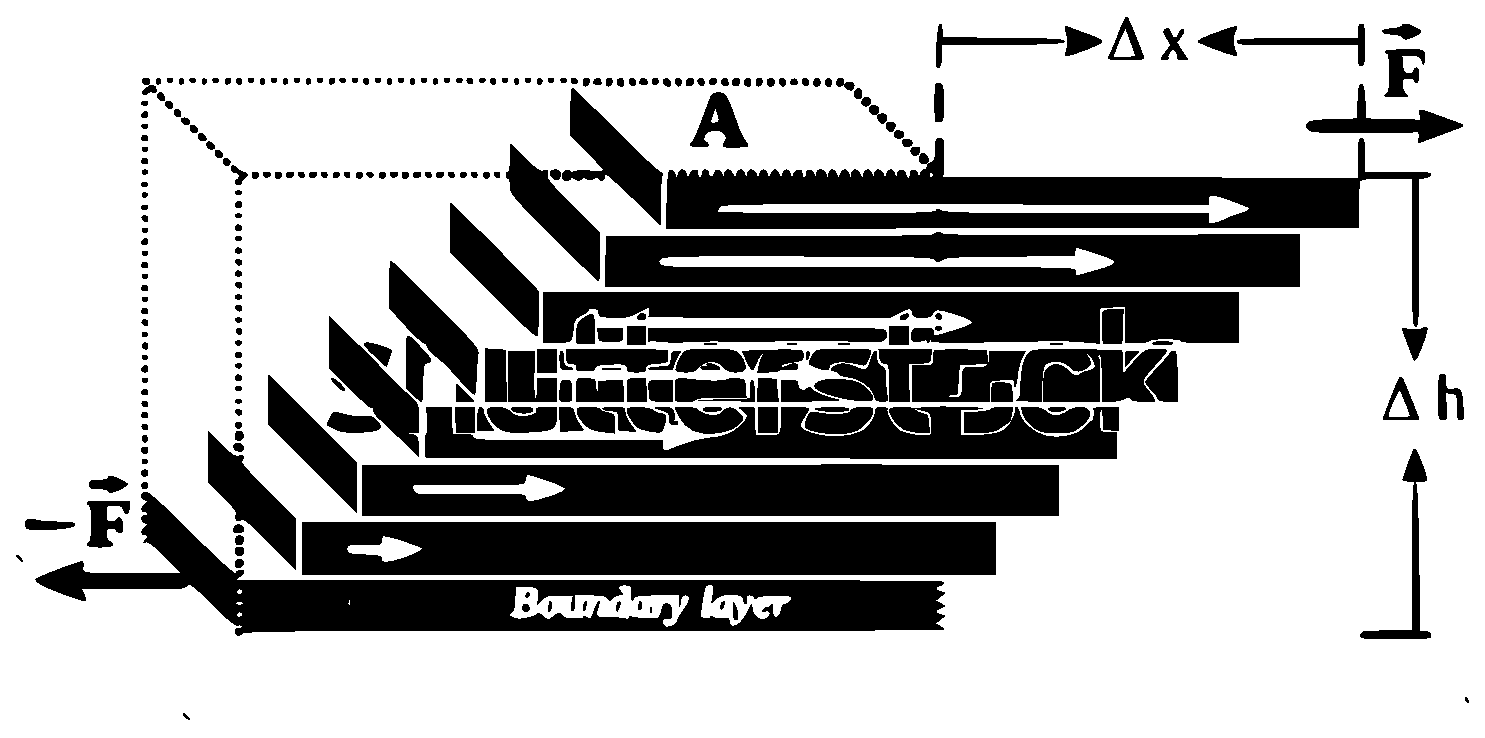
\includegraphics[scale=0.6]{me20b017.eps}
	\end{center}
\caption{Viscosity between the layers of a fluid}
\label{fig:viscous}
\end{figure}

\subsubsection{Terms used in the equation}
\begin{itemize}
	\item F - Viscous Force
	\item $\eta$ - viscosity of fluid
	\item A - Area of each plate
	\item $\frac{\partial v}{\partial z}$ - Velocity gradient 
\end{itemize}

\subsubsection{Importance of Viscous Force}
Viscous Force obtained using Equation~\ref{eqn:viscous} helps us to find 
out the viscous force existing between two surfaces. Viscosity is a kind 
of friction which exists between fluids. As shown in Figure .~\ref{fig:viscous}
each layer of a fluid experiences different viscous force compared to 
other.
%me20b017 end
